\documentclass[11pt]{article}
\usepackage{amsmath,amsthm, amssymb, latexsym,bm}
\usepackage{bbm}
\usepackage{algorithm}% http://ctan.org/pkg/algorithm
\usepackage{algorithmic}
\newcommand{\numpy}{{\tt numpy }}    % tt font for numpy
\usepackage{graphicx}

\usepackage{listings}
\usepackage{xcolor}
\definecolor{codegreen}{rgb}{0,0.6,0}
\definecolor{codegray}{rgb}{0.5,0.5,0.5}
\definecolor{codepurple}{rgb}{0.58,0,0.82}
\definecolor{backcolour}{rgb}{0.95,0.95,0.92}
\lstdefinestyle{mystyle}{
    backgroundcolor=\color{backcolour},
    commentstyle=\color{codegreen},
    keywordstyle=\color{magenta},
    numberstyle=\tiny\color{codegray},
    stringstyle=\color{codepurple},
    basicstyle=\ttfamily\footnotesize,
    breakatwhitespace=false,
    breaklines=true,
    captionpos=b,
    keepspaces=true,
    numbers=left,
    numbersep=5pt,
    showspaces=false,
    showstringspaces=false,
    showtabs=false,
    tabsize=2
}
\lstset{style=mystyle}


\topmargin -.5in
\textheight 9in
\oddsidemargin -.25in
\evensidemargin -.25in
\textwidth 7in

\begin{document}

% ========== Edit your name here
\author{Bruce Chappell}
\title{MAT 4110 Obligatory Assignment 1}
\maketitle

\medskip

% ========== Begin answering questions here
\begin{enumerate}
\section{Theory}
In this assignment I will study image compression using the SVD decomposition. Grey-scale images of size $[N \times M]$ will be studied. The images can be represented by a matrix $\bm{A}_{ij}$ where $i \in [0,N-1]$ and $j \in [0,M-1]$. \\
\\
An $[N \times M]$ matrix can bet decomposed into the form
\begin{equation}
    \bm{A} = \bm{U\Sigma V^{T}}
\end{equation}
Where $\bm{U}$ is an $[N \times N]$ orthogonal matrix, $\bm{V^{T}}$ is an $[M \times M]$ orthogonal matrix, and $\bm{\Sigma}$ is an $[N \times M]$ matrix with the singular values of $\bm{A}$ on the diagonal and zeros elsewhere. These singular values take the form
\begin{equation}
    \sigma_1 \geq \sigma_2 \geq \sigma \geq \dots \sigma_{N}
\end{equation}
$\sigma_i = \sqrt{\lambda_i}$ where $\lambda_i$ is the $i$th eigen value of the matrix $A^T A$. Since $\bm{U}$ and $\bm{V^T}$ are orthognal, they correspond to rotations and/or reflections of the $N$ and $M$ dimensional spaces. This means that the singular values are solely responsible for stretching or shrinking the vectors. This can be thought of as bigger values of $\Sigma$ explain more of the variance in $\bm{A}$, while smaller values explain less and are therefore less important.
\\
\\
We can find the variance explained by each singular vector of the SVD decomposition by computing
\begin{equation}
    R_i^2 = \frac{\sigma_i^2}{\sum_j \sigma_j^2}
\end{equation}
and plotting over the amount of singular vectors. This provides a nice visual to see when the singular values stop contributing significantly to the variance in $\bm{A}$. We can then make a choice to condense the information in the matrix by throwing out the singular values after a given $\sigma_{k}$ and then reconstructing $\bm{A}$ with $\bm{U}^{(n \times k)}$, $\bm{\Sigma}^{(k \times k)}$, and $\bm{V^T}^{(k \times m)}$.
\\
The compressed image can be characterized by the compression ratio which is give by
\begin{equation}
    \texttt{ratio} = \frac{\texttt{uncompressed size}}{\texttt{compressed size}} = \frac{M\times N}{K\times(1+M+N)}
\end{equation}
\\
\section{Results}
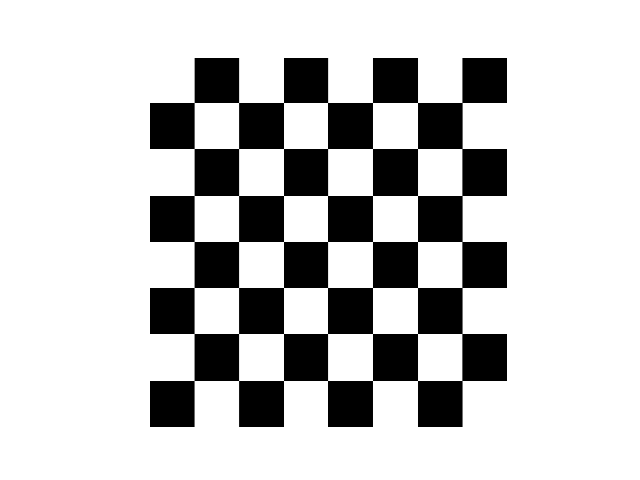
\includegraphics[scale=.55]{chess_g.png}
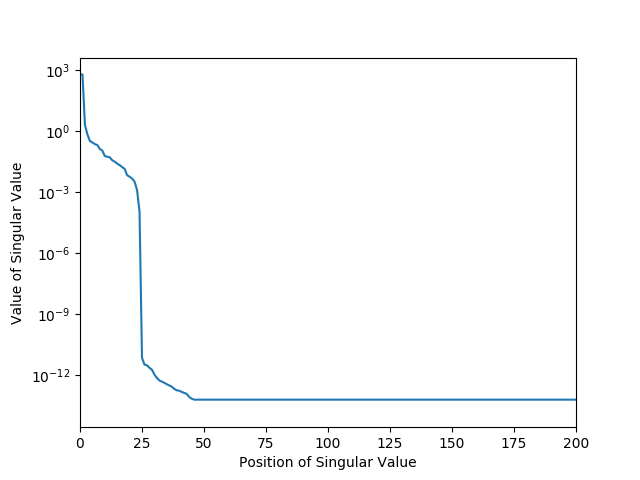
\includegraphics[scale=.55]{checker_sv.png}\\
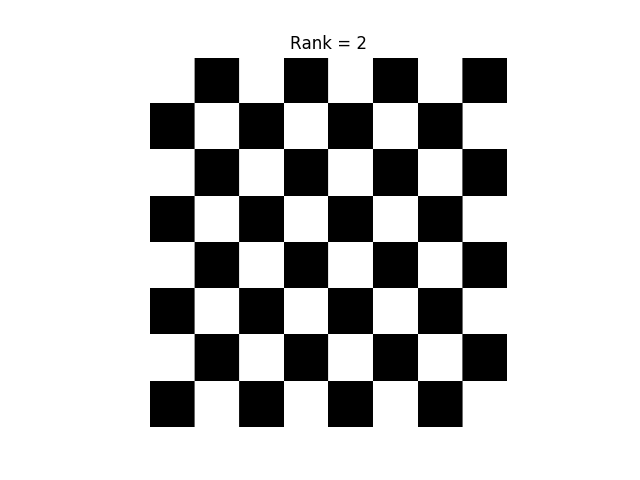
\includegraphics[scale=.55]{checker_compress.png}
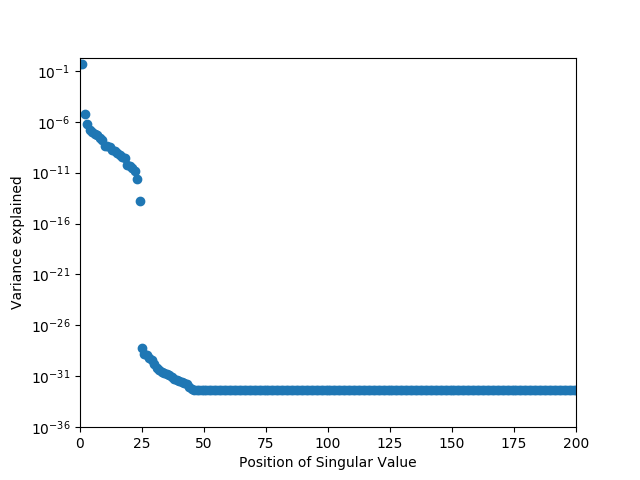
\includegraphics[scale=.55]{checker_var.png}\\
The original image is shown in the top left corner. From the two plots on the right, we see that the first singular value is the main contributor to the variance in the image and with just using the first two singular values we reproduce the image. Here, our compression ratio for the $1280 \times 1236$ image is $314.3$\\
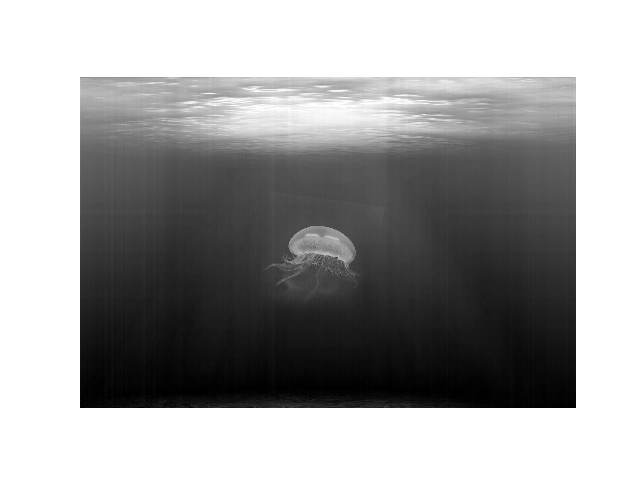
\includegraphics[scale=.55]{jelly_g.png}
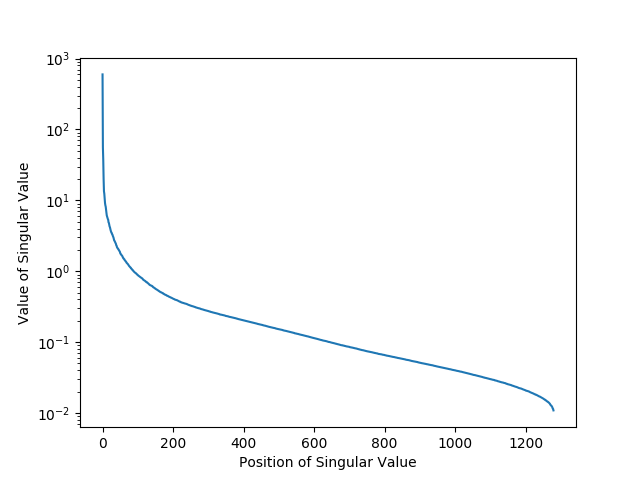
\includegraphics[scale=.55]{jelly_sv.png}\\
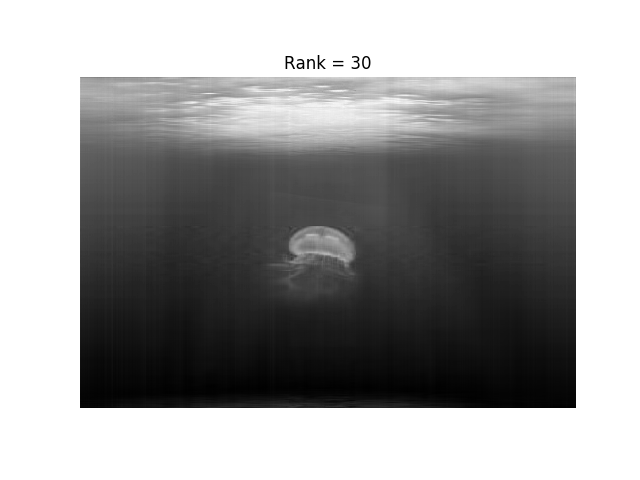
\includegraphics[scale=.55]{jelly_compress_30.png}
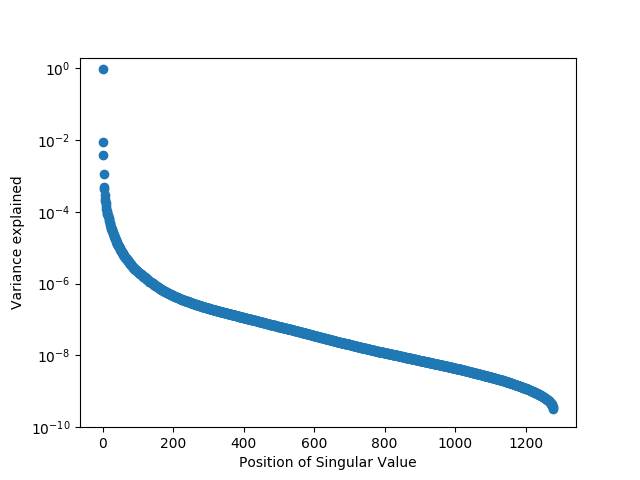
\includegraphics[scale=.55]{jelly_var.png}\\
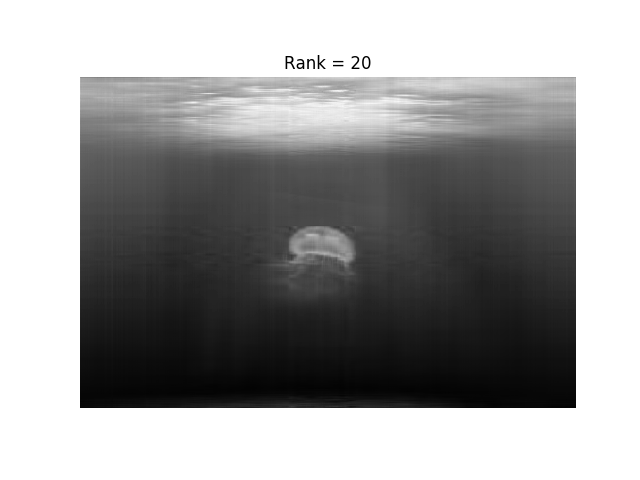
\includegraphics[scale=.55]{jelly_compress_20.png}\\
Compared to the checker board, this jellyfish has a larger number of significant singular values as the variance and singular value plot evolve more smoothly with respect to rank. For this image, I decided that rank 20 was not quite sharp enough and decided to go with rank 30. The compression ratio for the $1280 \times 1920$ image is $25.6$\\
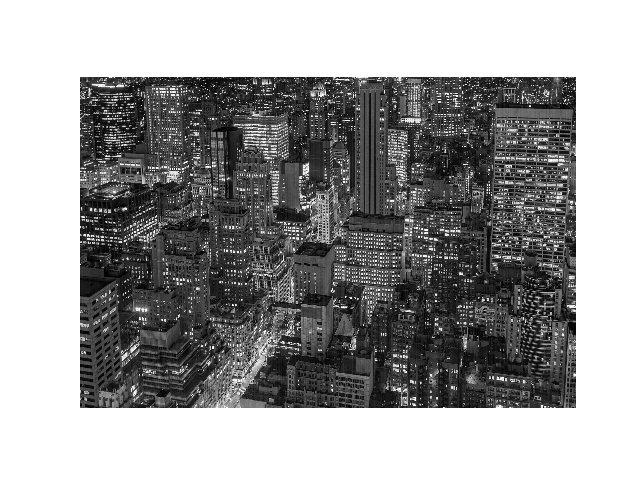
\includegraphics[scale=.55]{ny_g.png}
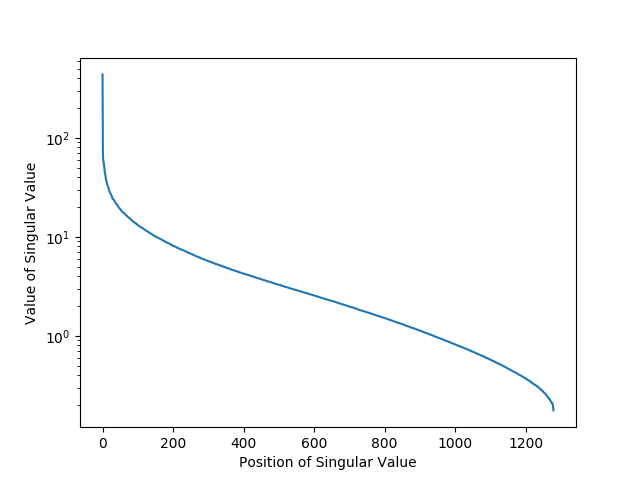
\includegraphics[scale=.55]{ny_sv.png}\\
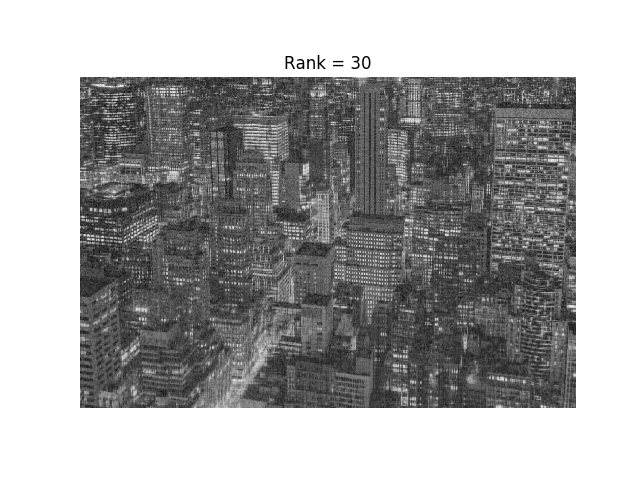
\includegraphics[scale=.55]{ny_compress_30.png}
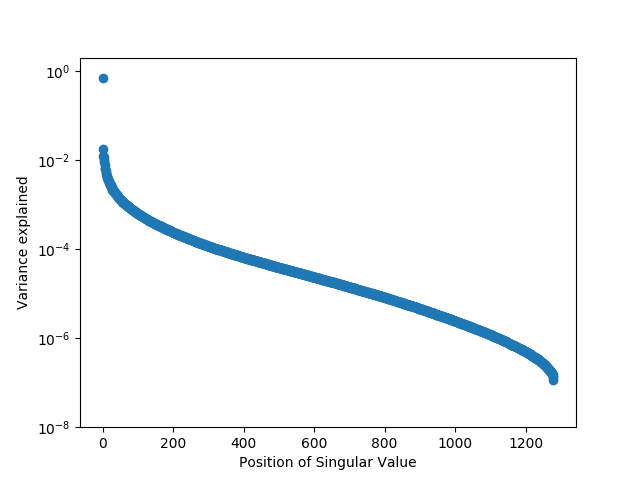
\includegraphics[scale=.55]{ny_var.png}\\
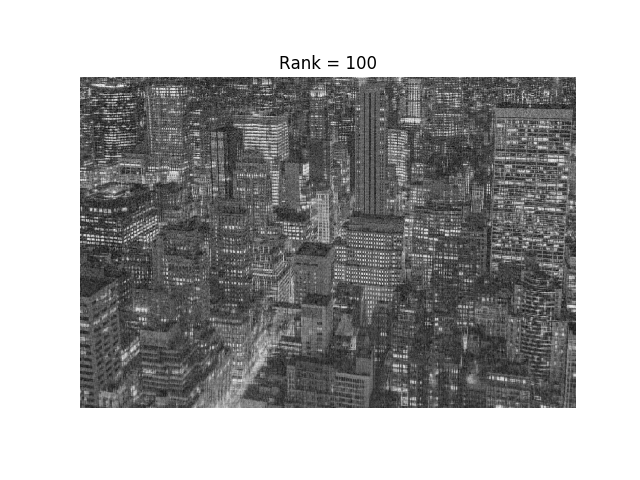
\includegraphics[scale=.55]{ny_compress_100.png}
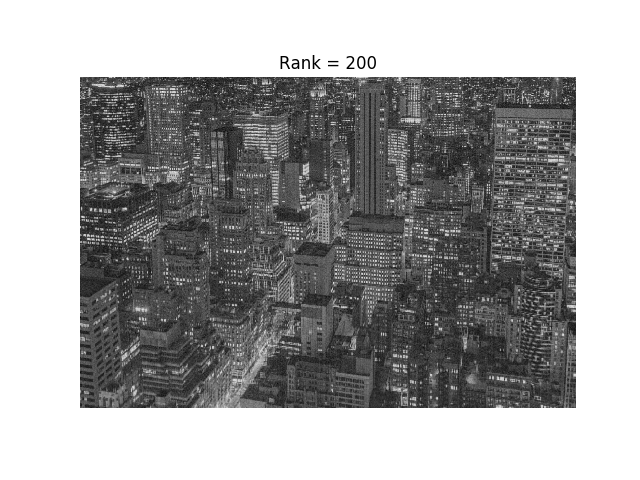
\includegraphics[scale=.55]{ny_compress_200.png}\\
Again, we find more singular values are needed to sharply reproduce the image. The smallest singular values in this image are larger than the smallest from the other images, meaning these values have more importance in this image. I decided that rank 200 produced a sharp enough reproduction resulting in a compression ratio of 3.8. It is clear that the more complex an image is, the more singular values you need to keep to reproduce it. As a result, the compression ratio for an appropriately condensed complex image is much smaller than that for a simple image.
\end{enumerate}

\begin{lstlisting}[language = Python]
from skimage import io
from skimage.color import rgb2gray
import numpy as np
from sklearn.preprocessing import MinMaxScaler
import matplotlib.pyplot as plt

# import and scale data
chess = io.imread('chess.png')
chess_g = rgb2gray(chess)

scaler = MinMaxScaler()
jelly = io.imread('jellyfish.jpg')
jelly_g = rgb2gray(jelly)
scaler.fit(jelly_g)
jelly_g = scaler.transform(jelly_g)

scaler1 = MinMaxScaler()
ny = io.imread('newyork.jpg')
ny_g = rgb2gray(ny)
scaler1.fit(ny_g)
ny_g = scaler1.transform(ny_g)

print(chess_g.shape, jelly_g.shape, ny_g.shape)

# show images
fig1, axes1 = plt.subplots()
axes1.imshow(jelly_g, cmap = plt.cm.gray)
axes1.axis('off')
plt.savefig('jelly_g')

fig2, axes2 = plt.subplots()
axes2.imshow(chess_g, cmap = plt.cm.gray)
axes2.axis('off')
plt.savefig('chess_g')

fig3, axes3 = plt.subplots()
axes3.imshow(ny_g, cmap = plt.cm.gray)
axes3.axis('off')
plt.savefig('ny_g')

def singular_val_study(image):
    u, s, vT = np.linalg.svd(image)
    val_vec = np.arange(s.shape[0])
    var = np.zeros_like(s)
    var = (s*s)/np.sum(s*s)
    return val_vec, s, var


def svd_compress(image, rank):
    u, s, vT = np.linalg.svd(image)
    s = s[:rank]
    u = u[:,:rank]
    vT = vT[:rank,:]
    print(u.shape)
    print(s.shape)
    print(vT.shape)
    compress = (u @ np.diag(s)) @ vT
    return rank, compress

# CHECKERS
range, s, var = singular_val_study(chess_g)
fig1 = plt.figure()
plt.semilogy(range,s)
plt.xlabel('Position of Singular Value')
plt.ylabel('Value of Singular Value')
plt.xlim(0,200)
plt.savefig('checker_sv')

fig2 = plt.figure()
plt.scatter(range,var)
plt.xlabel('Position of Singular Value')
plt.ylabel('Variance explained')
plt.yscale('log')
plt.xlim(0,200)
plt.ylim(1e-36,2*1e0)
plt.savefig('checker_var')
plt.show()

rank, n_checker = svd_compress(chess_g, 2)
fig = plt.figure()
plt.imshow(n_checker, cmap=plt.cm.gray)
plt.axis('off')
plt.title('Rank = 2')
plt.savefig('checker_compress')
plt.show()

# JELLY FISH
range, s, var = singular_val_study(jelly_g)
fig1 = plt.figure()
plt.semilogy(range,s)
plt.xlabel('Position of Singular Value')
plt.ylabel('Value of Singular Value')
plt.savefig('jelly_sv')

fig2 = plt.figure()
plt.scatter(range,var)
plt.xlabel('Position of Singular Value')
plt.ylabel('Variance explained')
plt.yscale('log')
plt.ylim(1e-10,2*1e0)
plt.savefig('jelly_var')
plt.show()

rank, n_jelly = svd_compress(jelly_g, 30)
fig = plt.figure()
plt.imshow(n_jelly, cmap=plt.cm.gray)
plt.axis('off')
plt.title('Rank = 30')
plt.savefig('jelly_compress_30')
plt.show()

#NYC
range, s, var = singular_val_study(ny_g)
fig1 = plt.figure()
plt.semilogy(range,s)
plt.xlabel('Position of Singular Value')
plt.ylabel('Value of Singular Value')
plt.savefig('ny_sv')

fig2 = plt.figure()
plt.scatter(range,var)
plt.xlabel('Position of Singular Value')
plt.ylabel('Variance explained')
plt.yscale('log')
plt.ylim(1e-8,2*1e0)
plt.savefig('ny_var')
plt.show()

rank, n_ny = svd_compress(ny_g, 200)
fig = plt.figure()
plt.imshow(n_ny, cmap=plt.cm.gray)
plt.axis('off')
plt.title('Rank = 200')
plt.savefig('ny_compress_200')
plt.show()
\end{lstlisting}
\end{document}
